\chapter{Design of the proposed solution}
\label{ch:DesignOfTheProposedSolution}
\lettrine[lraise=-0.1, lines=2, loversize=0.2]{T}{his} Chapter provides the details about the implementation of the solution to the problem in Chapter \ref{ch:ProblemFormulation}: block diagram, pseudocode and inter-module communications. All the code is available online~\footnote{Human aware collaboration planner source code: \url{https://github.com/grvcTeam/aerialcore_planning}}, and was developed under the Ubuntu 18.04 operating system and ROS Melodic.

The solution proposed follows a hierarchical approach, with a high-level planner in charge of activating different low-level controllers. The high-level planner detects the tasks required by the operators, and distributes them from the ground in a centralised way among the available \glspl{ACW}, planning the necessary recharges throughout the mission. In addition, this planner reacts in real time to possible events by reassigning tasks. The low-level planners are on board each \gls{UAV} and are responsible for executing contingency plans for these events while the central planner calculates and communicates the new plan. They will also be in charge of controlling the movement of the \glspl{ACW} to execute the different tasks assigned by the higher-level module (e.g., flying to a location to be inspected or to the position of an operator waiting for a tool). From now on, the low-level module on board each \gls{UAV} will be called the \emph{Agent Behaviour Manager}, and the centralised module on the ground will be called the \emph{High-Level Planner}. Together, these modules will provide cognitive capabilities to interact with humans efficiently in a dynamic scenario. 

%%%%%% ATENTION %%%%%%%%%%%%%
% (\emph{No se si quitar esta última frase, este párrafo es adaptado del proyecto de tesis})

\section{Block diagram}
\label{sec:NodeDiagram}
%% Informe de actividades: Node Diagram
As stated in Chapter \ref{ch:Introduction}, the developed task planner is part of a software architecture consisting of different layers, being the main cognitive block the central layer, the \emph{high-level cognitive task planner}. Figure \ref{fig:NodeDiagram} shows a schematic of the software architecture from the perspective of the module implemented in this thesis, including the different blocks and their interfaces. The part of the diagram in grey would be the complete software architecture, including from the high-level module in charge of analysing the gestures made by the operators to extract the tasks from them, to the low-level controllers in charge of executing those tasks. The software layer corresponding to this thesis, in charge of high-level decision-making, is marked in blue-green. It is composed of the \emph{High-Level Planner}, which is centralised and runs on a ground station (in orange) and the \emph{Agent Behaviour Manager}, distributed on board each \gls{ACW} (in lime).

\begin{figure}[ht]
    \hspace{-1cm}
	\scalebox{0.7}{
		\begin{tikzpicture}
    		% WP7 block
    		\node (WP7-Box) at (8.35,0) [fill=gray!15,rounded corners, draw=black!70, densely dotted, minimum height=5cm, minimum width=19.5cm]{}; 

			% Task planner box
    		\node (TaskPlannerBox) at ($(WP7-Box)+(0,0)$) [fill=teal!15,rounded corners, draw=black!70, densely dotted, minimum height=4.5cm, minimum width=14cm]{};
    		
    		% Gesture Recognition
    		\node (GestureRecognition) at (0,0) [text centered, fill=white, draw, rectangle, minimum width=1.5cm, text width=5.5em]{Gesture\\Recognition};
    		
    		\draw[-latex] ($(GestureRecognition) - (1.8,0)$) -- (GestureRecognition);
 
    		% High-Level Planner
    		\node (HighLevelPlannerBox) at ($(GestureRecognition) + (3.5,0.25)$) [fill=orange!15,rounded corners, draw=black!70, densely dotted, minimum height=2cm, minimum width=2.5cm]{}; 
    		\node (HighLevelPlanner) at ($(HighLevelPlannerBox) + (0,-0.25)$) [text centered, fill=white, draw, rectangle, minimum width=1.5cm, text width=5.5em]{High-Level\\Planner};
    		\node (Centralised) at ($(HighLevelPlanner) + (0,0.75)$) [text centered]{\small Centralised};
    		
    		\draw[-latex] (GestureRecognition.east) -- node[above]{Task} (HighLevelPlanner);
    		
    		%%%%%%%%%%%%%%%%%%%
    		% UAV 1
    		\node (UAV1) at ($(HighLevelPlanner) + (6.75,1.25)$) [fill=lime!20,rounded corners, draw=black!70, densely dotted, minimum height=1.7cm, minimum width=5cm]{}; 
    		\node (AgentBehaviourManager1) at ($(UAV1) + (0,-0.25)$) [fill=white, draw, rectangle, text centered, text width=12em]{Agent Behaviour Manager};
    		\node (UAV1-Text) at ($(AgentBehaviourManager1) + (0,0.75)$) [text centered]{\small On board ACW-$1$};	

    		\draw[fill=black] ($ (HighLevelPlanner.east) + (1.715,0) $) arc(-180:180:0.05);
    		\draw[-latex] (HighLevelPlanner.east) -- ($ (HighLevelPlanner.east) + (1.75,0) $) -- ($ (HighLevelPlanner.east) + (1.75,1) $) -- node[above]{Task} node[below]{List} (AgentBehaviourManager1.west);
    		\draw[-latex] ($ (HighLevelPlanner.east) + (1.75,0) $) -- node[above]{Feedback} (HighLevelPlanner.east);
    		
    		%%%%%%%%%%%%%%%%%%%
    		
    		% Dots
    		\node (Dots2) at ($(UAV1) + (0,-1.25)$) [text centered]{\dots};
    		
    		%%%%%%%%%%%%%%%%%%%
    		
    		% UAV N
    		\node (UAVN) at ($(HighLevelPlanner) + (6.75,-1.25)$) [fill=lime!20,rounded corners, draw=black!70, densely dotted, minimum height=1.7cm, minimum width=5cm]{}; 
    		\node (AgentBehaviourManagerN) at ($(UAVN) + (0,-0.25)$) [fill=white, draw, rectangle, text centered, text width=12em]{Agent Behaviour Manager};
    		\node (UAVN-Text) at ($(AgentBehaviourManagerN) + (0,0.75)$) [text centered]{\small On board ACW-$N$};	

    		\draw[-latex] (HighLevelPlanner.east) -- ($ (HighLevelPlanner.east) + (1.75,0) $) -- ($ (HighLevelPlanner.east) + (1.75,-1.5) $) -- node[above]{Task} node[below]{List} (AgentBehaviourManagerN.west);
    		
    		%%%%%%%%%%%%%%%%%%%
    		
    		% Lower-Level Controllers
    		\node (LowerLevelControllers) at ($(HighLevelPlanner) + (13.25,0)$) [text centered, fill=white, draw, rectangle, minimum width=1.5cm, text width=5.5em]{Lower-Level\\Controllers};
    		
    		\draw[-latex] (LowerLevelControllers.east) -- ($(LowerLevelControllers) + (1.8,0)$);
    		
    		\draw[fill=black] ($ (LowerLevelControllers.west) + (-1.535,0) $) arc(-180:180:0.05);
    		\draw[-latex] (AgentBehaviourManager1.east) -- ($ (LowerLevelControllers.west) + (-1.5,1) $) -- ($ (LowerLevelControllers.west) + (-1.5,0) $) --  node[above]{Task}
    	    node[below]{Params}	(LowerLevelControllers.west);
    		\draw[-latex] (LowerLevelControllers.west) -- ($ (LowerLevelControllers.west) + (-1.5,0) $) -- ($ (LowerLevelControllers.west) + (-1.5,1) $) -- node[above]{Task}
    	    node[below]{Result}	(AgentBehaviourManager1.east);
    		\draw[-latex] (AgentBehaviourManagerN.east) -- ($ (LowerLevelControllers.west) + (-1.5,-1.5) $) -- ($ (LowerLevelControllers.west) + (-1.5,0) $) -- (LowerLevelControllers.west);
    		\draw[-latex] (LowerLevelControllers.west) -- ($ (LowerLevelControllers.west) + (-1.5,0) $) -- ($ (LowerLevelControllers.west) + (-1.5,-1.5) $) -- 
    		node[above]{Task}
    		node[below]{Result} (AgentBehaviourManagerN.east);
    		
    		%%%%%%%%%%%%%%%%%%%%%
    		
    		\node (RealUAVs) at ($(WP7-Box.south) + (2,-1.25)$) [text centered, fill=white, draw, rectangle, minimum width=1.5cm, text width=6em]{ACWs\\autopilot};
    		\node (Humans) at ($(WP7-Box.south) + (-2,-1.25)$) [text centered, fill=white, draw, rectangle, minimum width=1.5cm, text width=6em]{Humans\\Tracker};
    		
    		\draw[-latex] (RealUAVs.north) -- node[right]{Pose, Battery, State} ($(WP7-Box.south) + (2,0)$);
    		\draw[-latex] ($(WP7-Box.south) + (2,0)$) -- (RealUAVs.north);
    		\draw[-latex] (Humans.north) -- node[left]{Pose} ($(WP7-Box.south) + (-2,0)$);
		
	    \end{tikzpicture}}
	\caption{Software architecture: blocks and interfaces. Block diagram from the high-level cognitive task planner perspective}
	\label{fig:NodeDiagram}
\end{figure}

In the software architecture scheme, although some communications are bidirectional, it can be seen that there is a main flow of information. Starting with the information arriving at the module \emph{Gesture Recognition}, this propagates to the last layer, where the \emph{Lower-Level Controllers} use the already processed information to command the \glspl{ACW}. Table \ref{tab:interfaces} shows the type of data that each of the modules in Figure \ref{fig:NodeDiagram} receives as input and the type of data that each of them sends as output. Additionally, Table \ref{tab:shareddata} explains the details of the data types. 

% Description of the data interfaces for each software module
\begin{table}[ht]
    \centering
    \caption{Description of the data interfaces for each software module}
    \label{tab:interfaces}
    \small
    \begin{tabular}{|p{0.25\columnwidth}|p{0.25\columnwidth}|p{0.4\columnwidth}|}
      \hline
      \multicolumn{1}{|c}{\textbf{Module Name}} & \multicolumn{1}{|c|}{\textbf{Input Data}} & \multicolumn{1}{c|}{\textbf{Output Data}}\\ \hline \hline
      Gesture Recognition & Images & \textbf{Task, defined by:} Task ID, Task Type, Monitoring Distance, Monitoring Number, WP List, Tool ID (some task parameters will be ignored depending on Task Type) \\ \hline
      
      High-Level Planner & Task, Feedback (Task Result, BatteryEnough, \gls{BT} info), Humans' Pose, \glspl{ACW}' Pose, Battery and State, and Agent Beacon & Task List adding to each one its extra parameters result of the planning (Formation and/or List of \glspl{ACW}' IDs) and Planner Beacon \\\hline
      
      Agent Behaviour Manager & Task List, Low-Level's Result, Human Pose, \glspl{ACW} Pose, Battery and State & Params needed by Low-Level Controllers (depending on Task Type), Feedback (Task Result, BatteryEnough, \gls{BT} info) and Agent Beacon \\ \hline
      
      Low-Level Controllers & Params (depending on Task Type) & Result \\ \hline
      
      Humans Tracker &  & Pose \\ \hline
      
      \gls{ACW} autopilot & Low-Level orders & Pose, Battery and State \\ \hline
      
    \end{tabular}
\end{table}

% Description of data types
\begin{table}[htb]
    \centering
    \caption{Description of data types}
    \label{tab:shareddata}
    \small
    \begin{tabular}{|p{0.2\columnwidth}|p{0.15\columnwidth}|p{0.55\columnwidth}|}
      \hline
      \multicolumn{1}{|c}{\textbf{Data name}} & \multicolumn{1}{|c|}{\textbf{Data type}} & \multicolumn{1}{c|}{\textbf{Comment}} \\ \hline \hline
      
      Task ID & String & Unique identifier of each task \\ \hline
      
      Task Type & Integer & Task type indicator: m/M, i/I or d/D \\ \hline
      
      Human Target ID & String & Unique identifier of each human worker. The position of the human target and other needed info is supposed to be known and accessible via its ID. \\ \hline
      
      Monitoring Distance & Float & Distance from which the \gls{ACW} surveil the worker during a safety monitoring task \\ \hline
      
      Monitoring Number & Integer & Number of \glspl{ACW} that are required in formation for a certain safety monitoring task \\ \hline
      
      WP List & List of $3$ float tuples ($x$, $y$, and $z$) & List of waypoints to be inspected \\ \hline
      
      List of \glspl{ACW}' IDs & List of Strings & List of the unique identifiers of the \glspl{ACW} that have been selected for a task that requires multiple \glspl{ACW} \\ \hline
      
      Formation & Integer & Indicates which of the predefined types of formations should be used for monitoring (e.g., circle, triangle) \\ \hline
      
      Tool ID & String & Unique identifier of the tool to be delivered \\ \hline
      
      \gls{ACW}'s Pose & geometry\_msgs /PoseStamped & \gls{ACW}'s Position and orientation \\ \hline
      
      \gls{ACW}'s Battery & sensors\_msgs /BatteryState & Percentage of battery in the \gls{ACW} \\ \hline

	  Task Result & String, Boolean & First one is the task unique \gls{ID} and second one its result once it's finished \\ \hline
      
      Battery Enough & Boolean & Result of computing if an \gls{ACW} will have enough battery for its current task \\ \hline

	  \gls{BT} info & String list & Status of each \gls{BT}'s node in its last execution (Running, IDLE, SUCCESS or FAILURE) \\ \hline
      
      Agent Beacon & String, String & First one is the \gls{ACW}'s unique ID while the second one defines \gls{ACW}'s type (SafetyACW, InspectACW, or PhysicalACW). It is used as heartbeat and to detect new \glspl{ACW} in Planner \\ \hline

	  Planner Beacon & Time & ROS::Time message containing the time when the beacon was sended. It is used to check the status of the connection from Agent's side. \\ \hline
      
      Lower-Level's Result & Boolean & Result of the Lower-Level Controllers once they have finished after being called \\ \hline
      
    \end{tabular}
\end{table}

The first module is constantly checking the images captured by the \glspl{UAV} for a gesture that is indicating a new task or the modification of an existing task. When this occurs, it asynchronously sends out a task, which will be picked up by the centralised planner. As shown in Table \ref{tab:interfaces}, this communication includes the unique \gls{ID} that differentiates this task from the others, the type of task, and the parameters that define it.

The \emph{High-Level Planner}, when it receives this information, proceeds to re-evaluate the optimal plan taking into account the task received, the information it receives from the \emph{\glspl{ACW}' autopilot}, and the position of the operators, which is periodically published by the \emph{Human Tracker}. These data constitute the input for the \emph{High-Level Planner}, together with the feedback coming from each \emph{Agent Behaviour Manager}. Its output is a list of tasks for each \gls{ACW}.

On board each \gls{ACW} there is an \emph{Agent Behaviour Manager}. This module is in charge of collecting the corresponding task list provided by the centralised planner. With this input and the information coming from the \emph{Human Tracker} and the \emph{\gls{ACW}'s autopilot}, this module is in charge of calling the \emph{Lower-Level Controllers} to carry out the execution of the assigned plan. The information emitted by the \emph{\gls{ACW}'s autopilot} is also used to check that everything is working correctly and to execute the security protocols in case they are necessary. If this happens, the corresponding communication would be issued back to the \emph{High-Level Planner} in order to calculate a new plan. Thes modules also receive the \emph{Lower-Level Controllers}' result after calling each of them, and publish it back to the \emph{High-Level Planner} as feedback.

In addition to these communications, the modules \emph{High-Level Planner} and \emph{Agent Behaviour Manager} periodically exchange beacons that are used to detect both the connection of a new \gls{ACW} and its disconnection in case of failure. Moreover, there is an asynchronous communication that is broadcast to all components indicating the end of the mission when this happens.

Finally, it is worth mentioning that the \emph{Gesture Recognition} module does not have a communication aimed at modifying parameters of a task already contemplated within the \emph{High-Level Planner}. However, this is possible because tasks have a unique identifier. Once a task has been delivered to the \emph{High-Level Planner}, in order to change any of its parameters, the \emph{Gesture Recognition} module just has to submit the task again, keeping the same task \gls{ID} and updating only the desired parameters. Thus, the \emph{High-Level Planner} could overwrite it and allocate it again with the new parameters.

\section{Centralised module: High-Level Planner}
\label{sec:Centralised module:TaskPlanner}
As mentioned above, the \emph{High-Level Planner} is a centralised module running on a ground station and constitutes the main cognitive module of the software architecture. Its purpose is to plan the mission in an optimal way, i.e., to distribute the pending tasks among the available \glspl{ACW} by specifying the order in which they are to be executed, taking into account the time it takes to complete each one, the type of each \glspl{UAV}, the distance each one will have to travel, the battery they have available, the task each one was executing, the priority of each task, the battery consumed by each task, the recharges that will be needed, and when it is best to carry out those recharges.

%% Explicación y Pseudocódigo general de como se inicializa el nodo planner, el bucle while(ros::ok) y como se cierra cuando mission_over. Incluir escucha a imprevistos.
The general pseudocode for this component from launch to termination is depicted in Code \ref{ps:GeneralPlanner}.

\begin{lstlisting}[caption={General operation of \emph{High-Level Planner}'s code}, breaklines=true, label=ps:GeneralPlanner]
	1. Read from a ros::param the address of the configuration file.
	2. Read from the configuration file all necessary information.
	3. Configure ROS communications (Publishers, Subscribers and ActionServers).
	4. Set the loop rate.
	5. Main "while" loop. While ros::ok() and not mission over do:
		5.1. Check the timeout of the Agents' beacons.
		5.2. Publish a new Planner beacon.
		5.3. Check for pending incoming communications (ros::spinOnce).
		5.4. Sleep the remaining time to send the next beacon.
	6. Wait until all UAVs have finished and disconnected. While there is any agent connected do:
		6.1. Check the timeout of the Agents' beacons.
		6.2. Check for pending incoming communications (ros::spinOnce).
		6.3. Sleep for a while.
\end{lstlisting}

%% Decir que todo funciona con callbacks y explicarlos. (batteryEnoughCB, taskResultCB, positionCallback, batteryCallback)(incomingTask, beaconCallback, missionOverCallback)
Since the environment in which the \glspl{UAV} operate is dynamic, this module has been programmed in such a way that it can react to unforeseen events and recalculate the optimal plan. As it can be deduced from Code \ref{ps:GeneralPlanner}, everything works through callback functions. Every time a communication arrives from another ROS node, a response is triggered on this node. The information contained in the message is analysed and it is decided whether a replanning is necessary or not. The situations in which a replanning has been deemed necessary are listed in Section \ref{sec:TaskReplanningSituations}. The communications summarised in Tables \ref{tab:interfaces} and \ref{tab:shareddata} and in Figure \ref{fig:NodeDiagram} are sufficient to detect these unforeseen events and to be able to respond to them in the best possible way.

\begin{lstlisting}[caption={Task callback pseudocode}, breaklines=true, label=ps:IncomingTask]
	1. Check if the task already exists and delete it in order to create it with the new parameters.
	2. Read the type of task and the parameters that apply to it.
	3. Add the new task to the pending task list.
	4. Perform a task planning.
\end{lstlisting}

There is a callback that is executed when the node \emph{Gesture Recognition} sends a task, which always ends up calling the function in charge of calculating the optimal plan (see Code \ref{ps:IncomingTask}); the mission over callback, whose only action is to change the value of a variable so that the node exits the main while loop; and finally the agent's beacon callback, which is executed every time a \gls{UAV} beacon is received and whose pseudocode is in Code \ref{ps:AgentBeaconCallback}.

\begin{lstlisting}[caption={Agent's beacon callback}, breaklines=true, label=ps:AgentBeaconCallback]
	1. Read the information contained in the beacon.
	2. If it is a connection of a new UAV:
		2.1. Register it in the database.
		2.2. Perform a task planning.
	3. Else, if it is the heartbeat of an already known UAV:
		3.1. Reset the timeout timer.
\end{lstlisting}

The action carried out by the agent's beacon callback varies depending on whether it is the beacon of a new \gls{UAV} or the heartbeat of a known \gls{UAV}. For each agent there will be an object in the database that will contain another series of callbacks that will be in charge of receiving the messages coming from the \glspl{ACW} and respond accordingly.

\begin{lstlisting}[caption={Callback that runs when an \emph{Agent Behaviour Manager} sends battery feedback}, breaklines=true, label=ps:batteryEnoughCB]
	1. Update the value of the internal flag associated with the battery.
	2. Perform a task planning.
\end{lstlisting}

The \emph{Agent Behaviour Manager} block only sends communications messages indicating the battery status when it is due to an unplanned event. This event can be either an early battery depletion or a faster than expected recharge. In both cases, the callback function, whose pseudocode is Code \ref{ps:batteryEnoughCB}, updates the value of an internal variable used during planning, and recalculates the optimal plan.

The other possible communication coming from a node of type \emph{Agent Behaviour Manager} with the ability to trigger a reaction in the planner is due to the termination of a task. When a task finishes successfully, it is simply removed from the list of pending tasks. In addition, this moment is used to re-evaluate the optimal plan. It is expected that the mission is still within the optimal plan, so in that case the planning result should be the same as the plan that was already being executed. If, instead, conditions have changed since the last planning and there exists a better plan now, it is at this point that the plan is updated. If the task ends with a failure, the callback action will depend on the causes of the failure (note that the interruption of a task will result in a failure). If the interruption is due to the \gls{UAV} battery, it may be planned, in which case no action is required, or it may be unexpected, in which case the corresponding actions are taken by the battery callback. Once it has been verified that the task has not finished due to the battery, a check is made to see if the task was at the beginning of the queue. If so, a failure has indeed occurred, so the operators are warned, the task is removed from the list, and a replanning is executed. Otherwise the task in question would have been moved from the top of the queue due to a change of plans and therefore no action would have to be taken either. The pseudocode corresponding to what has just been explained is in Code \ref{ps:taskResultCB}.

\begin{lstlisting}[caption={Callback that runs when an \emph{Agent Behaviour Manager} sends a task result}, breaklines=true, label=ps:taskResultCB]
	1. Read the information contained in the task result.
	2. If the task result is SUCCESS:
		2.1. Delete it from the pending tasks list.
		2.2. Perform a task planning.
	3. Else, if the task result is FAILURE:
		3.1. If the task has been halted because of not having battery enough:
			3.1.1. Return.
		3.2. Else, if the task is on the front of that ACW's task queue:
			3.2.1. Notify operators that a task has failed and is going to be deleted.
			3.2.2. Delete task from the pending tasks list.
			3.2.3. Perform a task planning.
		3.3. Else:
			3.3.1. Return.
\end{lstlisting}

The other two communications received by the \emph{High-Level Planner} from the \glspl{ACW} are sensor readings corresponding to the \glspl{UAV}' position and battery percentage. In both cases the only action of the corresponding callback is to update the information with the new values.

The last function that remains to be explained of those that can potentially request a replanning of the mission is the one in charge of checking the timeout of the agents' beacons. As shown in  Code \ref{ps:GeneralPlanner}, this function is not a callback like the previous ones, instead it is executed periodically in the main while loop. Its operation is shown in Code \ref{ps:checkBeaconsTimeout}. Basically, for each agent connected, it checks that the timeout amount of time has not elapsed since its last beacon was received. If a timeout has occurred, that \gls{ACW} is considered disconnected and is removed from the centralised node data. If, after checking all agents, the number of connected \glspl{UAV} has decreased, i.e. if any of the previously connected \glspl{UAV} has disconnected, a mission replanning is executed.

% Pseudocódigo de checkBeaconsTimeout
\begin{lstlisting}[caption={Beacons' timeout check function}, breaklines=true, label=ps:checkBeaconsTimeout]
	1. For each agent connected:
		1.1. If the elapsed time since the last beacon is greater than the timeout time:
			1.1.1. Add that agent's ID to the list of disconnected agents.
	2. While the list of disconnected agents is not empty:
		2.1. Take first ID from the list.
		2.2. Erase from the block's data all information related to that ID.
	3. If any agent has been disconnected:
		3.1. Perform a task planning.
\end{lstlisting}

%% Explicar como se realiza la planificación y poner psudocódigo de cómo se lleva a cabo. Explicar también como se calcula el coste.
The pseudocode that is executed when one of these functions deems it necessary to perform a new task planning is summarised in Code \ref{ps:performTaskAllocation}. It is important to remember that some tasks have a higher priority than others, and this depends only on the type of task. To simplify the process, it has been decided to allocate the tasks in order of arrival, assuming that between two tasks of the same type, the one that arrived first will have priority. When a new task is received, it is stored both in a \emph{std::map} that contains all the pending tasks to facilitate the access to the information, and in a \emph{std::vector} with task types, where the order of arrival is maintained. What this simplification allows is to assign tasks one at a time. By having a prioritised list of tasks and assuming that no task can be assigned before a task with a higher priority, the mission planning problem is reduced to calculating the cost of each task individually for each \gls{UAV} with the ability to execute it and assign it to the one with the lowest cost. For monitoring-type tasks, the selection of the required number of agents is strictly cost-based. The \emph{N} agents that cost the least to execute the task are selected. The same is a little more complex for the tasks of type inspect, where the number of agents to select is a parameter to be defined by the planner itself. This value is first set according to the number of points to be inspected. Up to three points, a single \gls{ACW} is selected; up to six points, two are selected; and from seven points onwards, three agents are selected, this being the maximum number imposed by the low-level controller. Moreover, as the low-level controller in charge of this task works, all the \glspl{ACW} selected for this task are required to start executing it simultaneously, so a second approximation of this number is made according to the number of idle \glspl{UAV}. Thus, if they are assigned this as the first task, they will start executing it simultaneously. Academically, this simplification seems to deviate from the optimal solution, but it should be recalled that this work is part of a software architecture that will operate in real situations. In such situations, it is not expected that there will be a large number of \glspl{UAV} connected simultaneously, nor a long list of pending tasks. In such simplified scenarios, this assumption makes sense without deviating too much from the optimal solution. Finally, the number of agents to be selected will be the smaller of the two above, being equal to one when there is no \gls{UAV} idle and zero in case there is no \gls{ACW} with enough battery. In the latter case, the task would be assigned after recharging. Once the number of agents to be selected has been defined, the agents that have the least cost to execute the task are selected from among those that meet the conditions described. Having selected the \gls{ACW} that will carry out the task, all that remains is to distribute among them the \glspl{WP} to be inspected. Although the algorithm in charge of performing the optimal distribution is in the low-level controller of this task, as the rest of the modules that make up the software architecture are not yet available, it has been necessary to program a distribution algorithm in order to be able to carry out the experiments. More details on this will be given in Section \ref{sec:faking}.

% Explicar como se calcula el coste.
The cost for each \gls{UAV} is calculated as the weighted sum of three different types of costs. A first cost assesses the type of \gls{ACW} and penalises the assignment of tasks to those \glspl{UAV} designed for another type. It penalises especially the assignment of lower priority tasks to agents designed to perform higher priority tasks. The second cost evaluates the total distance the \gls{UAV} will have to travel from where it is at the beginning of the task to where it should be by the end of the task. This cost is an approximation of the expected battery consumption, although it does not take into account intermediate travel and hoovering times during the mission. The last cost penalises the interruption of the task that was being executed according to the previous plan and rewards the assignment of the same task. This cost is intended to ensure that a task is preferentially assigned to an idle \gls{UAV}, to an \gls{UAV} that is executing a lower priority task, or even to an \gls{UAV} of a different type, rather than interrupting a task unnecessarily just because that \gls{ACW} has to travel a shorter distance, for example.

\begin{lstlisting}[caption={Task planning function's pseudocode}, breaklines=true, label=ps:performTaskAllocation]
	1. If there is any agent connected:
		1.1. For each agent connected:
			1.1.1. Make a copy of the current task queue.
			1.1.2. Empty the task queue.
		1.2. For each Tool Delivery task:
			1.2.1. Compute the cost of the task for each PhysicalACW that has enough battery.
			1.2.2. Assign the task to the agent for whom the task costs the least (from those who has enough battery).
			1.2.3. Add the task to that agent's task queue.
		1.3. For each Inspection task:
			1.3.1. Extract from the task parameters the list of WP to inspect.
			1.3.2. For each ACW (any type) that has enough battery:
				1.3.2.1. Compute the cost of the task for that ACW. 
				1.3.2.2. Check if that ACW is still idle.
			1.3.3. Calculate the number of agents to select for the task based on the number of WP and the number of idle agents.
			1.3.4. If no agent has enough battery, continue.
			1.3.5. Else, if the number of agents to select is equal to zero, assign the task to the agent that costs the least.
			1.3.6. Else, select the calculated number of agents for whom the task costs the least.
			1.3.7. Divide the WP to inspect among the selected agents.
			1.3.8. For each selected agent:
				1.3.8.1. Set the remaining task parameters (List of selected ACWs' IDs and divided WP list).
				1.3.8.2. Add the task to the agent's task queue.
		1.4. For each Monitoring task:
			1.4.1. Compute the cost of the task for each ACW (any type) that has enough battery.
			1.4.2. If the required number of ACWs for the task is zero:
				1.4.2.1. Warn operators that this parameter can not be zero.
				1.4.2.2. Delete task from pending tasks.
			1.4.3. Else, select the requested number of agents for whom the task costs the least.
			1.4.4. Set the remaining task parameter (List of selected ACWs' IDs)
			1.4.4. Add the task to each selected agent's task queue.
		1.5. For each ACW connected, send the new task queue to its Agent Behaviour Manager.
	2. Else:
		2.1. Warn operators that no agent is connected.
\end{lstlisting}

Once the calculation of the mission plan has been completed, the new task queues are sent to the corresponding distributed modules. Each \emph{Agent Behaviour Manager} will react to this communication and will take care of executing the newly assigned plan. In the meantime, the \emph{High-Level Planner} block returns to the main while loop to continue waiting until an event that triggers a replanning occurs again.

\section{Distributed module: Agent Behaviour Manager}
\label{sec:Distributed module: behaviour manager}
%% Explicar qué es una drone behavior manager y cual es su función.
This component is in charge of executing the plan assigned by the \emph{High-Level Planner}, checking the security of the \glspl{UAV} at all times, detecting unforeseen events and communicating them to the centralised node so that it can make a change of plans if needed. The \emph{Agent Behaviour Manager} will communicate with the low-level controllers, handing over control when necessary to complete the assigned plan.

%% Estructura general del nodo (pseudocodigo). Explicar que se ha hecho con árboles de comportamiento en paralelo a algunos procesos de ros
The general structure of this module is quite similar to that of the central module. The pseudocode is summarised in Code \ref{ps:GeneralAgent}. Upon initialisation, the \emph{Agent Behaviour Manager} prepares the necessary information to start its operation, configures the necessary communications, declares and initialises the behaviour tree and, once the \gls{UAV} has finished initialising, starts sending beacons to the central node to notify that it is joining the mission. Once the code finishes initialising and reaches the main while loop, the activity of the \emph{Agent Behaviour Manager} concentrates on the execution of callbacks in response to incoming messages, as in the \emph{High-Level Planner}, and on the execution of the behaviour tree, which directs and supervises the \gls{UAV} movement.

\begin{lstlisting}[caption={General operation of \emph{Agent Behaviour Manager}}, breaklines=true, label=ps:GeneralAgent]
	1. Read from a ros::param the beacon's content (ACW's ID and type).
	2. Read from a ros::param the address of the configuration file.
	3. Read from the configuration file all necessary information.
	4. Configure ROS communications (Publishers, Subscribers and ActionServers).
	5. Set the loop rate.
	6. Declare the behaviour tree.
	7. Initialise each BT node.
	8. Start BT loggers to facilitate debugging and monitoring of the node's performance.
	9. Wait until the ACW fully initialises.
	10. Main "while" loop. While ros::ok() and BT status is running:
		10.1. If a timeout of Planner's beacons has not ocurred:
			10.1.1. Publish a new Agent beacon.
		10.2. Check if battery is enough for the current task.
		10.3. Check for pending incoming communications (ros::spinOnce).
		10.4. Sleep the remaining time to send the next beacon.
\end{lstlisting}

%% Explicar lo que es un árbol de comportamiento y compararlo con una máquina de estados.
The \glspl{BT} are who governs the \glspl{ACW} to perform each of the assigned tasks. Each \gls{BT} monitors its \gls{ACW}'s battery and task status and reacts to any possible failure or unexpected event, requesting a new re-planning to the \emph{High-Level Planner} in case of need. A \gls{BT} can be defined as an improved \gls{FSM}. They are a more advanced mechanism to implement behaviours, especially because of their advantages in terms of scalability, modularity, readability and reusability, facilitating the creation of more complex behaviours with less effort.

%% Diseño del árbol de comportamiento.
Despite this, the process of designing a state machine is quite different from the process of designing a behaviour tree. Designing behaviour trees without ever having done it before is not a trivial task. Moreover, there will be more than one valid implementation to achieve the same behaviour, which makes it more complicated to design this type of solution when you do not still have enough intuition to know which one is better. Taking advantage of the fact that the use of \glspl{BT} is widespread in the videogame industry, information about them was gathered and studied to try to develop enough knowledge and intuition to design from scratch a \gls{BT} that meets the needs of the mission. For that, previous examples found in \cite{BT-CPP-doc, colledanchise2018behavior, BT-AI} were very useful.

Before proceeding with the explanation of the designed \gls{BT}, the types of nodes that can be found in the selected C++ library (see Figure~\ref{fig:BTnodes}) and the functioning of each of them will be briefly discussed.

%% Tipos de nodos de BT
\begin{figure}[htbp]
    \centering
    \subfloat[]{%Fallback
		\label{subfig:Fallback}
        
\begin{tikzpicture}
			\node (MainTree) at (0,0) [text centered, fill=white, draw, rectangle, minimum width=0.5cm, text width=0.5em]{\textbf{?}};
		\end{tikzpicture}}
    \hfill
    \subfloat[]{%Sequence
		\label{subfig:Sequence}
        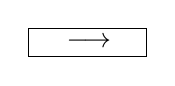
\begin{tikzpicture}
			\node (MainTree) at (0,0) [text centered, fill=white, draw, rectangle, minimum width=1.5cm, text width=1.5em]{$\longrightarrow$};
		\end{tikzpicture}}
	\hfill
    \subfloat[]{%Reactive
		\label{subfig:Reactive}
        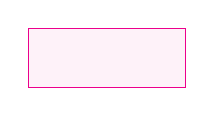
\begin{tikzpicture}
			\node (MainTree) at (0,0) [text centered, fill=magenta!5, draw=magenta, rectangle, minimum width=2cm, minimum height=0.75cm, text width=2em]{};
		\end{tikzpicture}}
    \hfill
    \subfloat[]{%Common
		\label{subfig:Common}
        \begin{tikzpicture}
			\node (MainTree) at (0,0) [text centered, fill=white, draw, rectangle, minimum width=2cm, minimum height=0.75cm, text width=2em]{};
		\end{tikzpicture}}
    \hfill
    \subfloat[]{%Decorator
		\label{subfig:Decorator}
        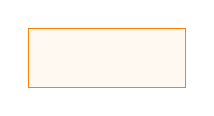
\begin{tikzpicture}
			\node (MainTree) at (0,0) [text centered, fill=orange!5, draw=orange, rectangle, minimum width=2cm, minimum height=0.75cm, text width=2em]{};
		\end{tikzpicture}}
    \hfill
    \subfloat[]{%Action
		\label{subfig:Action}
		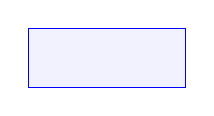
\begin{tikzpicture}
			\node (MainTree) at (0,0) [text centered, fill=blue!5, draw=blue, rectangle, minimum width=2cm, minimum height=0.75cm, text width=2em]{};
		\end{tikzpicture}}
		\hfill
    \subfloat[]{%Condition
		\label{subfig:Condition}
        \begin{tikzpicture}
			\node (MainTree) at (0,0) [text centered, fill=blue!5, draw=blue, ellipse, minimum width=2cm, minimum height=0.75cm, text width=2em]{};
		\end{tikzpicture}}
    \caption{Different types of nodes that can be present in an \gls{BT}}
    \label{fig:BTnodes}
\end{figure}

 Behaviour Trees are made up of \emph{Control} nodes, \emph{Decorator} nodes, and \emph{Leaf} nodes. \emph{Control} nodes could be either \emph{Fallback} nodes, represented with a question mark (see subfigure \ref{subfig:Fallback}), which try success calling one by one each of their children; or \emph{Sequence} nodes, represented with an arrow (see subfigure \ref{subfig:Sequence}), which call their children in order if the previous one has succeeded. On the one hand, \emph{Fallback} nodes return \emph{SUCCESS} if one of its children does it, \emph{FAILURE} if none of them success, and \emph{RUNNING} if one of its children returns \emph{RUNNING}. On the other hand, \emph{Sequence} nodes return \emph{SUCCESS} when all children have been called in order and have returned \emph{SUCCESS}. If any of them returns \emph{FAILURE}, the sequence is broken and the \emph{Sequence} node returns \emph{FAILURE} too. When a child returns \emph{RUNNING}, the \emph{Sequence} node does it too. \emph{Control} nodes are represented in a black rectangular box when they are the standard ones (see subfigure \ref{subfig:Common}), but they could also be \emph{Reactive} control nodes, represented by a magenta box (see subfigure \ref{subfig:Reactive}), which means that its already called children will be called again in the next iteration. This is very useful for generating behaviours where an action is constantly reattempted, or where it is necessary to check that the required conditions are still met. A \emph{Child} node could be another \emph{Control} node, a \emph{Decorator} node, a \emph{Leaf} node or a whole sub-tree. A \emph{Decorator} node, represented in an orange box (see subfigure \ref{subfig:Decorator}), can only have one child (of any type) and its function is programmable (e.g., modifying its child result or retrying calling its child a number of times). \emph{Leaf} nodes, represented in blue, could be \emph{Condition} nodes, represented in a blue elliptical shaped box (see subfigure \ref{subfig:Condition}), that check a condition and return either \emph{SUCCESS} or \emph{FAILURE}; or \emph{Action} nodes, represented in a blue rectangular box (see subfigure \ref{subfig:Action}), that execute code that takes longer and therefore these nodes could also return \emph{RUNNING}.

\subsection{Main tree}
\label{sec:MainTree}
In general, the design of both the behaviour tree and the \emph{Agent Behaviour Manager} has been made with the aim of concentrating as less intelligence as possible, to ensure the success of the mission and the safety of the \glspl{UAV} and the workers. That is why the only task of the callback functions that are executed when different messages come in is to update the value of the corresponding internal variables. 

However, not all intelligence and decision-making can be placed in the ground station node. There has to be some decision-making capability on board \glspl{UAV} in case the connection to the central node is lost. That is why there is a predefined protocol to act when this happens or when the battery runs out of power earlier than expected. These two factors are periodically checked in the main while loop (see Code \ref{ps:GeneralAgent}). In the case of the battery, if the function in charge determines that there is not enough battery to complete the current task, what happens is that the task queue is emptied and the value of the internal flag associated with the battery is updated. In addition, the event is communicated to the task planner in case the connection is still alive to generate a new plan. Similarly, if a connection loss is detected, the task queue is emptied and the corresponding flag is updated. In this case the \emph{High-Level Planner} node will execute a replanning when it also detects the connection loss.

The behaviour tree is designed in such a way that, when the task queue is emptied and the respective flags are updated, the corresponding \gls{UAV} goes to the battery charging station, which is the established emergency protocol. In order to justify this decision, each of the cases will be analysed separately below.

In case the connection between the two nodes is still active but there is not enough battery, the aim of the contingency plan is to eliminate risks to the \gls{UAV} while the \emph{High-Level Planner} generates new instructions. In addition, the new plan is likely to involve recharging the battery as a first step. Besides, there is a possibility that the connection may be lost at this point.

The danger of connection loss is that the \emph{High-Level Planner} will replan the mission without the disconnected \gls{ACW}, so that the tasks previously assigned to it will now be executed by others. If in this scenario the disconnected \gls{ACW} continues with the last assigned plan, collisions could occur. The emergency protocol ensures that the disconnected \gls{UAV} does not interfere with the new plans. In addition, the time until the connection is re-established is used by recharging the battery, which is positive for the mission.

%%%%%%%%%%%%%%%%%%% El Agent Behavior Manager no elimina nunca una tarea de la cola en la revión actual. ¿Eso lo omito o debería explicarlo?

\glspl{BT} operate recursively. All nodes, regardless of their type, have a function that executes their content, the \emph{tick} function. When the root node is \emph{ticked} from the main while loop, it propagates the \emph{tick} among its children following the operation rules described in Section \ref{sec:Distributed module: behaviour manager} until eventually a \emph{leaf} node returns one of three possible responses (\emph{SUCCESS}, \emph{RUNNING} or \emph{FAILURE}), which will be propagated back, to obtain a final result that the root node will return. 

Typically, a \gls{BT} is executed to achieve a goal, and therefore the executor keeps on doing \emph{tick} to the tree root until the response is either \emph{SUCCESS} or \emph{FAILURE}. As the function of this \gls{BT} is to control during the whole mission the movement of a \gls{UAV}, it is of interest that the result of the root is \emph{RUNNING} until the mission ends. This is why a \emph{Decorator} node that always returns \emph{RUNNING} regardless of the result of its child node has been defined. The \gls{BT} implemented as a solution for the described problem is further divided into several \glspl{BT}, taking advantage of the modularity offered by this approach. The main tree is represented in Figure \ref{fig:MainTree}, being the node named as \emph{Main Tree} the root of the complete tree.

\begin{figure}[ht]
	\begin{center}
		\scalebox{0.9}{
			\begin{tikzpicture}
        		\node (MainTree) at (0,0) [text centered, fill=white, draw, rectangle, minimum width=1.5cm, text width=5.5em]{Main Tree};

        		\node (RootFallback) at ($(MainTree) + (0,-1)$) [text centered, fill=magenta!5, draw=magenta, rectangle, minimum width=0.5cm, text width=0.5em]{\textbf{?}};
        		\draw[-latex] (MainTree.south) -- (RootFallback.north);

        		\node (MissionOverSequence) at ($(RootFallback) + (-3,-1.5)$) [text centered, fill=white, draw, rectangle, minimum width=1.5cm, text width=1.5em]{$\longrightarrow$};
        		\draw[-latex] (RootFallback.south) -- (MissionOverSequence.north);
        		\node (ForceRunning) at ($(RootFallback) + (3, -1.5)$) [text centered, fill=orange!5, draw=orange, rectangle, minimum width=1.5cm, text width=5.5em]{Force Running};
        		\draw[-latex] (RootFallback.south) -- (ForceRunning.north);
        		
        		\node (MissionOver) at ($(MissionOverSequence) + (-1.75,-1.5)$) [text centered, fill=blue!5, draw=blue, ellipse, minimum width=1.5cm, text width=5.5em]{Mission Over?};
        		\draw[-latex] (MissionOverSequence.south) -- (MissionOver.north);
        		\node (BackToStation) at ($(MissionOverSequence) + (1.75, -1.5)$) [text centered, fill=blue!5, draw=blue, rectangle, minimum width=1.5cm, text width=5.5em]{Back To Station};
        		\draw[-latex] (MissionOverSequence.south) -- (BackToStation.north);
        		\node (MissionFallback) at ($(ForceRunning) + (0,-1.5)$) [text centered, fill=magenta!5, draw=magenta, rectangle, minimum width=0.5cm, text width=0.5em]{\textbf{?}};
        		\draw[-latex] (ForceRunning.south) -- (MissionFallback.north);

        		\node (IdleSequence) at ($(MissionFallback) + (-4.25,-1.25)$) [text centered, fill=magenta!5, draw=magenta, rectangle, minimum width=1.5cm, text width=1.5em]{$\longrightarrow$};
        		\draw[-latex] (MissionFallback.south) -- (IdleSequence.north);
        		\node (WaitFallback) at ($(MissionFallback) + (4.25,-1.25)$) [text centered, fill=magenta!5, draw=magenta, rectangle, minimum width=0.5cm, text width=0.5em]{\textbf{?}};
        		\draw[-latex] (MissionFallback.south) -- (WaitFallback.north);
        		
        		\node (Inverter) at ($(IdleSequence) + (-3, -1.5)$) [text centered, fill=orange!5, draw=orange, rectangle, minimum width=1.5cm, text width=5.5em]{Inverter};
        		\draw[-latex] (IdleSequence.south) -- (Inverter.north);
        		\node (TaskSequence) at ($(IdleSequence) + (2.5,-1.5)$) [text centered, fill=magenta!5, draw=magenta, rectangle, minimum width=1.5cm, text width=1.5em]{$\longrightarrow$};
        		\draw[-latex] (IdleSequence.south) -- (TaskSequence.north);
        		\node (IsBatteryFull) at ($(WaitFallback) + (-1.75,-1.5)$) [text centered, fill=blue!5, draw=blue, ellipse, minimum width=1.5cm, text width=5.5em]{Is Battery Full?};
        		\draw[-latex] (WaitFallback.south) -- (IsBatteryFull.north);
        		\node (Recharge) at ($(WaitFallback) + (1.75, -1.5)$) [text centered, fill=blue!5, draw=blue, rectangle, minimum width=1.5cm, text width=6.5em]{Recharge};
        		\draw[-latex] (WaitFallback.south) -- (Recharge.north);

        		\node (Idle) at ($(Inverter) + (0,-1.5)$) [text centered, fill=blue!5, draw=blue, ellipse, minimum width=1.5cm, minimum height=1.35cm, text width=5.5em]{Idle?};
        		\draw[-latex] (Inverter.south) -- (Idle.north);
        		\node (IsBatteryEnough) at ($(TaskSequence) + (-1.75,-1.5)$) [text centered, fill=blue!5, draw=blue, ellipse, minimum width=1.5cm, text width=5.5em]{Is Battery Enough?};
        		\draw[-latex] (TaskSequence.south) -- (IsBatteryEnough.north);
        		\node (PerformTaskTree) at ($(TaskSequence) + (1.75, -1.5)$) [text centered, fill=white, draw, rectangle, minimum width=1.5cm, text width=6.5em]{Perform Task Tree};
        		\draw[-latex] (TaskSequence.south) -- (PerformTaskTree.north);
        		
        		%\draw[-latex] (.south) -- (.north);
		    \end{tikzpicture}}
		\caption{Behaviour Tree: Main tree}
		\label{fig:MainTree}
	\end{center}
	\vspace{-1em}
\end{figure}

This \gls{BT} checks whether the mission is over (reminder: a mission would represent the working session, not a single task, i.e., whether the \gls{ACW} is ready to be turned off) and if so directs the \gls{ACW} back to the base station. If not, the main \emph{Fallback} ticks to the right branch of the tree, entering the \emph{Recursive Fallback} node that controls the mission. This branch checks if any tasks are assigned. If it turns out that the \gls{ACW} is idle and the battery is not at hundred percent, the \gls{ACW} is guided to a recharging station~\footnote{Both Safety, Inspection and Physical-ACW provide an input interface to guide the \gls{ACW} to the charging station. In other words, among the low-level controller capabilities, there is a "reach this waypoint". The location of the charging stations is known in advance or provided as input by the High-Level Planner/Behaviour Tree.}. If a task is assigned and the corresponding flag indicates that the battery is enough, it enters directly into the \emph{Perform Task Tree} (sub-tree represented in Figure~\ref{fig:PerformTasksTree}).

This \emph{Recursive Fallback} is where is coded the behaviour that prepares the \gls{BT} to be safe against a loss of connection or an unexpected battery event. As both unexpected events are managed flushing the task queue, the \gls{ACW} reacts recharging, while giving the High-Level Planner control to decide when it is the best time to stop recharging (the High-Level Planner just needs to assign tasks again so that the \gls{ACW} starts working back). Note that, thanks to the presence of \emph{Recursive Control} nodes, the \emph{Leaf Condition} nodes are constantly being re-evaluated. Thus, in case of any unforeseen event or change of plan, the \gls{BT} will react by instantly stopping the executing branch and switching to the appropriate branch.

\begin{figure}[ht]
	\begin{center}
		\scalebox{0.75}{
			\begin{tikzpicture}
			    \node (PerformTaskTree) at (0,0) [text centered, fill=white, draw, rectangle, minimum width=1.5cm, text width=5.5em]{Perform Task Tree};
        		
        		\node (TaskFallback) at ($(PerformTaskTree) + (0,-1.5)$) [text centered, fill=magenta!5, draw=magenta, rectangle, minimum width=0.5cm, text width=1.5em]{\textbf{?}};
        		\draw[-latex] (PerformTaskTree.south) -- (TaskFallback.north);
        		
        		\node (MonitorSequence) at ($(TaskFallback) + (-7,-1.5)$) [text centered, fill=magenta!5, draw=magenta, rectangle, minimum width=1.5cm, text width=1.5em]{$\longrightarrow$};
        		\draw[-latex] (TaskFallback.south) -- (MonitorSequence.north);
        		\node (InspectSequence) at ($(TaskFallback) + (0,-1.5)$) [text centered, fill=magenta!5, draw=magenta, rectangle, minimum width=1.5cm, text width=1.5em]{$\longrightarrow$};
        		\draw[-latex] (TaskFallback.south) -- (InspectSequence.north);
        		\node (DeliverSequence) at ($(TaskFallback) + (7,-1.5)$) [text centered, fill=magenta!5, draw=magenta, rectangle, minimum width=1.5cm, text width=1.5em]{$\longrightarrow$};
        		\draw[-latex] (TaskFallback.south) -- (DeliverSequence.north);
        		
        		\node (IsTaskMonitor) at ($(MonitorSequence) + (-1.75,-2)$) [text centered, fill=blue!5, draw=blue, ellipse, minimum width=1.5cm, text width=6em]{Is Task "Monitoring"?};
        		\draw[-latex] (MonitorSequence.south) -- (IsTaskMonitor.north);
        		\node (MonitorTree) at ($(MonitorSequence) + (1.75, -2)$) [text centered, fill=white, draw, rectangle, minimum width=1.5cm, text width=6.5em]{Monitoring Task Tree};
        		\draw[-latex] (MonitorSequence.south) -- (MonitorTree.north);
        		\node (IsTaskInspect) at ($(InspectSequence) + (-1.75,-2)$) [text centered, fill=blue!5, draw=blue, ellipse, minimum width=1.5cm, text width=5.5em]{Is Task "Inspection"?};
        		\draw[-latex] (InspectSequence.south) -- (IsTaskInspect.north);
        		\node (InspectTree) at ($(InspectSequence) + (1.75, -2)$) [text centered, fill=white, draw, rectangle, minimum width=1.5cm, text width=5.5em]{Inspection Task Tree};
        		\draw[-latex] (InspectSequence.south) -- (InspectTree.north);
        		\node (IsTaskDeliver) at ($(DeliverSequence) + (-1.75,-2)$) [text centered, fill=blue!5, draw=blue, ellipse, minimum width=1.5cm, text width=5.5em]{Is Task "Tool Delivery"?};
        		\draw[-latex] (DeliverSequence.south) -- (IsTaskDeliver.north);
        		\node (DeliverTree) at ($(DeliverSequence) + (1.5, -2)$) [text centered, fill=white, draw, rectangle, minimum width=1.5cm, text width=6.5em]{Tool Delivery Task Tree};
        		\draw[-latex] (DeliverSequence.south) -- (DeliverTree.north);
        		
		    \end{tikzpicture}}
		\caption{Behaviour Tree: Perform Task Tree}
		\label{fig:PerformTasksTree}
	\end{center}
\end{figure}

The \emph{Perform Task Tree} checks which is the first task in the queue, which is the task that should be executed at that moment. This tree does not require much more explanation, it simply connects the \emph{Main Tree} with the corresponding \emph{Task sub-tree}. At this point, instead of sub-trees, it would be possible to directly place \emph{Leaf} nodes that give control to the appropriate low-level controller, starting to execute the task directly. However, it was decided that the full control would not be given to the low-level controllers until the \gls{ACW} is close enough to the area where the task takes place.

In Figures \ref{fig:MonitorTree}, \ref{fig:InspectTree} and \ref{fig:DeliverToolTree} are depicted the sub-trees that run Safety, Inspection, and Physical tasks, respectively. They all guide the \gls{ACW} close enough to where the low-level controllers need to be called (e.g., close to a worker to monitor or a place to inspect) and then, control is given to the corresponding one. These low-level controllers run on board the corresponding \glspl{ACW} and communicate their results (success or failure) asynchronously back to the \emph{Agent Behaviour Manager}, so that the \gls{BT} can continue running.

In the following, the functioning of each of these sub-trees is described, as well as the details of each of the tasks that have not yet been explained.

\subsection{Inspection task tree}
\label{sec:InspectionTaskTree}
This \gls{BT} is quite simple as the task is just to visit a series of points and stop at each one to take pictures (see Fig. \ref{fig:InspectTree}).

\begin{figure}[ht]
	\begin{center}
		\scalebox{0.9}{
			\begin{tikzpicture}
			    \node (InspectTree) at (0,0) [text centered, fill=white, draw, rectangle, minimum width=1.5cm, text width=5.5em]{Inspection Task Tree};
        		
        		\node (InspectTaskSequence) at ($(InspectTree) + (0,-1.5)$) [text centered, fill=magenta!5, draw=magenta, rectangle, minimum width=1.5cm, text width=1.5em]{$\longrightarrow$};
        		\draw[-latex] (InspectTree.south) -- (InspectTaskSequence.north);
        		
        		\node (NearWPFallback) at ($(InspectTaskSequence) + (-1.5,-1.5)$) [text centered, fill=magenta!5, draw=magenta, rectangle, minimum width=0.5cm, text width=0.5em]{\textbf{?}};
        		\draw[-latex] (InspectTaskSequence.south) -- (NearWPFallback.north);
        		\node (Inspect) at ($(InspectTaskSequence) + (1.5,-1.5)$) [text centered, fill=blue!5, draw=blue, rectangle, minimum width=1.5cm, text width=5.5em]{Inspect};
        		\draw[-latex] (InspectTaskSequence.south) -- (Inspect.north);
        		
        		\node (IsUAVnearWP) at ($(NearWPFallback) + (-1.75,-2)$) [text centered, fill=blue!5, draw=blue, ellipse, minimum width=1.5cm, text width=5.5em]{Is \gls{ACW} near WP?};
        		\draw[-latex] (NearWPFallback.south) -- (IsUAVnearWP.north);
        		\node (GoNearWP) at ($(NearWPFallback) + (1.75, -2)$) [text centered, fill=blue!5, draw=blue, rectangle, minimum width=1.5cm, text width=6.5em]{Go near WP};
        		\draw[-latex] (NearWPFallback.south) -- (GoNearWP.north);
		    \end{tikzpicture}}
		\caption{Behaviour Tree: sub-tree that controls the inspection tasks}
		\label{fig:InspectTree}
	\end{center}
\end{figure}

As mentioned above, control is handed over to the low-level controllers when the \gls{ACW} is close enough to the area where the task takes place. The \emph{Reactive Sequence Control} node behind the root of this sub-tree is in charge of checking this condition at any moment, stopping the low-level controller if it is no longer fulfilled.

All the information that the \gls{BT} needs to operate is known in advance by the \emph{Agent Behaviour Manager}, either because it has received it through one of the interfaces represented in Figure \ref{fig:NodeDiagram}, or because it has calculated it itself in one of the functions that are executed in the main while loop. In particular, to check if the \gls{ACW} is close to the points to be inspected, the information received from the \emph{\gls{ACW}'s autopilot} is used against the points in the list of \glspl{WP} to be inspected. If necessary, the \emph{Action} node \emph{Go near \gls{WP}} is executed, which connects to the low-level controller in charge and gives as target location the nearest \gls{WP} in the list. Once there, the low-level controller that executes this task is called.

\subsection{Monitoring task tree}
\label{sec:MonitoringTaskTree}
As can it be seen in Figure \ref{fig:MonitorTree}, this \gls{BT} follows the same structure as the previous one. The only differences are the \emph{Leaf} nodes.

\begin{figure}[ht]
	\begin{center}
		\scalebox{0.9}{
			\begin{tikzpicture}
			    \node (MonitorTree) at (0,0) [text centered, fill=white, draw, rectangle, minimum width=1.5cm, text width=5.5em]{Monitoring Task Tree};
        		
        		\node (MonitorTaskSequence) at ($(MonitorTree) + (0,-1.5)$) [text centered, fill=magenta!5, draw=magenta, rectangle, minimum width=1.5cm, text width=1.5em]{$\longrightarrow$};
        		\draw[-latex] (MonitorTree.south) -- (MonitorTaskSequence.north);
        		
        		\node (NearHumanFallback) at ($(MonitorTaskSequence) + (-1.5,-1.5)$) [text centered, fill=magenta!5, draw=magenta, rectangle, minimum width=0.5cm, text width=1.5em]{\textbf{?}};
        		\draw[-latex] (MonitorTaskSequence.south) -- (NearHumanFallback.north);
        		\node (MonitorHumanTarget) at ($(MonitorTaskSequence) + (1.5,-1.5)$) [text centered, fill=blue!5, draw=blue, rectangle, minimum width=1.5cm, text width=5.5em]{Monitor};
        		\draw[-latex] (MonitorTaskSequence.south) -- (MonitorHumanTarget.north);
        		
        		\node (IsUAVnearHumanTarget) at ($(NearHumanFallback) + (-2,-2)$) [text centered, fill=blue!5, draw=blue, ellipse, minimum width=1.5cm, text width=6.5em]{Is \gls{ACW} near Human Target?};
        		\draw[-latex] (NearHumanFallback.south) -- (IsUAVnearHumanTarget.north);
        		\node (GoNearHuman) at ($(NearHumanFallback) + (1.55, -2)$) [text centered, fill=blue!5, draw=blue, rectangle, minimum width=1.5cm, text width=6.5em]{Go near Human Target};
        		\draw[-latex] (NearHumanFallback.south) -- (GoNearHuman.north);
		    \end{tikzpicture}}
		\caption{Behaviour Tree: sub-tree that controls the safety monitoring tasks}
		\label{fig:MonitorTree}
	\end{center}
	\vspace{-1em}
\end{figure}

In this case, the position of the operator to be monitored is known from communications with the \emph{Human Tracker} node (see Figure \ref{fig:NodeDiagram}). If the \gls{ACW} is not close enough, the \gls{BT} will call the low-level controller giving it this time the position of the operator as a target. Once the \gls{UAV} is in a position close to the worker, control is passed to the low-level controller in charge of this task. The information needed by this node is the \emph{Monitoring Number}, the \emph{Monitoring Distance}, the \emph{list of \glspl{ACW}' \glspl{ID}}, and the formation to be maintained during the flight, which will be chosen by the \emph{High-Level Planner} from a set of predefined formations based on the monitoring number (see Table \ref{tab:shareddata}). Finally, it is worth mentioning that an \gls{ACW} could be added or removed from the formation at any time by updating the parameters of the task, or even due to availability.

\subsection{Tool delivery task tree}
\label{sec:ToolDeliveryTaskTree}
This tree is a bit more complex, as the task involves several steps (see Fig. \ref{fig:DeliverToolTree}). First, it picks up the requested tool in case the \gls{ACW} does not have it yet. This part involves travelling to the station to pick up the tool in case the \gls{UAV} is not already there. The second part of the task is the process of approaching the operator. After all this, the low-level controller can be activated to carry out the delivery of the tool through a physical interaction between the operator and the \gls{ACW}.

\begin{figure}[ht]
	\begin{center}
		\scalebox{0.85}{
			\begin{tikzpicture}
			    \node (DeliverTree) at (0,0) [text centered, fill=white, draw, rectangle, minimum width=1.5cm, text width=6.5em]{Tool Delivery Task Tree};
			    
			    \node (DeliverTaskSequence) at ($(DeliverTree) + (0,-1)$) [text centered, fill=magenta!5, draw=magenta, rectangle, minimum width=1.5cm, text width=1.5em]{$\longrightarrow$};
        		\draw[-latex] (DeliverTree.south) -- (DeliverTaskSequence.north);

				\node (ToolFallback) at ($(DeliverTaskSequence) + (-6.5,-1.5)$) [text centered, fill=magenta!5, draw=magenta, rectangle, minimum width=0.5cm, text width=0.5em]{\textbf{?}};
        		\draw[-latex] (DeliverTaskSequence.south) -- (ToolFallback.north);
        		\node (HumanFallback) at ($(DeliverTaskSequence) + (0,-1.5)$) [text centered, fill=white, draw, rectangle, minimum width=0.5cm, text width=0.5em]{\textbf{?}};
        		\draw[-latex] (DeliverTaskSequence.south) -- (HumanFallback.north);
        		%\node (PermissionFallback) at ($(DeliverTaskSequence) + (6.5,-1.5)$) [text centered, fill=magenta!5, draw=magenta, rectangle, minimum width=0.5cm, text width=0.5em]{\textbf{?}};
        		%\draw[-latex] (DeliverTaskSequence.south) -- (PermissionFallback.north);
				\node (DeliverTool) at ($(DeliverTaskSequence) + (3.5,-1.5)$) [text centered, fill=blue!5, draw=blue, rectangle, minimum width=1.5cm, text width=6.5em]{Deliver Tool};
        		\draw[-latex] (DeliverTaskSequence.south) -- (DeliverTool.north);

				\node (hasACWtheTool) at ($(ToolFallback) + (-1.5,-2)$) [text centered, fill=blue!5, draw=blue, ellipse, minimum width=1.5cm, text width=5.5em]{Has \gls{ACW} the Tool?};
        		\draw[-latex] (ToolFallback.south) -- (hasACWtheTool.north);
        		\node (PickToolSequence) at ($(ToolFallback) + (1.5,-2)$) [text centered, fill=magenta!5, draw=magenta, rectangle, minimum width=1.5cm, text width=1.5em]{$\longrightarrow$};
        		\draw[-latex] (ToolFallback.south) -- (PickToolSequence.north);
        		\node (IsUAVnearHuman) at ($(HumanFallback) + (-1.75,-2)$) [text centered, fill=blue!5, draw=blue, ellipse, minimum width=1.5cm, text width=6.5em]{Is \gls{ACW} near Human Target?};
        		\draw[-latex] (HumanFallback.south) -- (IsUAVnearHuman.north);
        		\node (GoNearHuman) at ($(HumanFallback) + (1.75, -2)$) [text centered, fill=blue!5, draw=blue, rectangle, minimum width=1.5cm, text width=6.5em]{Go near Human Target};
        		\draw[-latex] (HumanFallback.south) -- (GoNearHuman.north);
        		%\node (DeliverSequence) at ($(PermissionFallback) + (-2.25,-2)$) [text centered, fill=white, draw, rectangle, minimum width=1.5cm, text width=1.5em]{$\longrightarrow$};
        		%\draw[-latex] (PermissionFallback.south) -- (DeliverSequence.north);
        		%\node (ForceFailure) at ($(PermissionFallback) + (2.25, -2)$) [text centered, fill=orange!5, draw=orange, rectangle, minimum width=1.5cm, text width=5.5em]{Force Failure};
        		%\draw[-latex] (PermissionFallback.south) -- (ForceFailure.north);


        		\node (StationFallback) at ($(PickToolSequence) + (-1.5,-2)$) [text centered, fill=white, draw, rectangle, minimum width=0.5cm, text width=0.5em]{\textbf{?}};
        		\draw[-latex] (PickToolSequence.south) -- (StationFallback.north);
        		\node (PickTool) at ($(PickToolSequence) + (1.5, -2)$) [text centered, fill=blue!5, draw=blue, rectangle, minimum width=1.5cm, text width=6.5em]{Pick Tool};
        		\draw[-latex] (PickToolSequence.south) -- (PickTool.north);
        		%\node (hasUAVpermission) at ($(DeliverSequence) + (-3.25,-2)$) [text centered, fill=white, draw, ellipse, minimum width=1.5cm, text width=5.5em]{Has  permission?};
        		%\draw[-latex] (DeliverSequence.south) -- (hasUAVpermission.north);
        		%\node (DeliverTool) at ($(DeliverSequence) + (0, -2)$) [text centered, fill=white, draw, rectangle, minimum width=1.5cm, text width=6.5em]{Tool Delivery};
        		%\draw[-latex] (DeliverSequence.south) -- (DeliverTool.north);
        		%\node (Retreat) at ($(DeliverSequence) + (3, -2)$) [text centered, fill=white, draw, rectangle, minimum width=1.5cm, text width=4.5em]{Retreat};
        		%\draw[-latex] (DeliverSequence.south) -- (Retreat.north);
        		%\node (WaitFallback) at ($(ForceFailure) + (0,-2)$) [text centered, fill=magenta!5, draw=magenta, rectangle, minimum width=0.5cm, text width=0.5em]{\textbf{?}};
        		%\draw[-latex] (ForceFailure.south) -- (WaitFallback.north);
        		
        		\node (IsUAVnearStation) at ($(StationFallback) + (-1.75,-2)$) [text centered, fill=blue!5, draw=blue, ellipse, minimum width=1.5cm, text width=5.5em]{Is \gls{ACW} near Station?};
        		\draw[-latex] (StationFallback.south) -- (IsUAVnearStation.north);
        		\node (GoNearStation) at ($(StationFallback) + (1.75, -2)$) [text centered, fill=blue!5, draw=blue, rectangle, minimum width=1.5cm, text width=6.5em]{Go near Station};
        		\draw[-latex] (StationFallback.south) -- (GoNearStation.north);
        		%\node (TimeoutSequence) at ($(WaitFallback) + (-1.5,-2)$) [text centered, fill=white, draw, rectangle, minimum width=1.5cm, text width=1.5em]{$\longrightarrow$};
        		%\draw[-latex] (WaitFallback.south) -- (TimeoutSequence.north);
        		%\node (Wait) at ($(WaitFallback) + (1.5, -2)$) [text centered, fill=white, draw, rectangle, minimum width=1.5cm, text width=6.5em]{Wait for Permission};
        		%\draw[-latex] (WaitFallback.south) -- (Wait.north);

        		%\node (Timeout) at ($(TimeoutSequence) + (-3.25,-2)$) [text centered, fill=white, draw, ellipse, minimum width=1.5cm, text width=5.5em]{Timeout?};
        		%\draw[-latex] (TimeoutSequence.south) -- (Timeout.north);
        		%\node (GoNearStation) at ($(TimeoutSequence) + (0, -2)$) [text centered, fill=white, draw, rectangle, minimum width=1.5cm, text width=6.5em]{Go near Station};
        		%\draw[-latex] (TimeoutSequence.south) -- (GoNearStation.north);
        		%\node (DropTool) at ($(TimeoutSequence) + (3.25, -2)$) [text centered, fill=white, draw, rectangle, minimum width=1.5cm, text width=6.5em]{Drop the Tool};
        		%\draw[-latex] (TimeoutSequence.south) -- (DropTool.north);
		    \end{tikzpicture}}
		\caption{Behaviour Tree: sub-tree that controls the tool delivery tasks}
		\label{fig:DeliverToolTree}
	\end{center}
\end{figure}

Again, the location of the operator and the position of the \gls{ACW} is provided by the \emph{\gls{ACW}'s autopilot} and \emph{Human Tracker} blocks. The position of the fixed elements, in this case, the station where the tools are placed, is available among the information read by the \emph{Agent Behaviour Manager} node from the configuration file during its initialisation.

In this case, the low-level controller that delivers the tool will be in charge of requesting the operator's permission to approach. In the meantime, it will have to wait. When it gets the permission, it is time to make the delivery. If too much time elapses without the operator giving the order, the task will be aborted and the tool will be returned to the station.

\section{High- and low-level blocks faking}
\label{sec:faking}
The work in this thesis consisted of programming one of the software layers that make up a software architecture. As there are still parts of the software architecture that are not yet available for integration, temporary solutions have had to be programmed to simulate their action during testing. This section will discuss those parts of the code whose mission is to fool both \emph{High-Level Planner} and \emph{Agent Behaviour Manager} blocks into believing that they are communicating with the real blocks, or to provide functions necessary for the execution to progress.

Low-level controllers have been faked in different ways. For \gls{BT}'s \emph{Action} nodes of the \emph{"Go To"} type, the \emph{GoToWaypoint} \gls{ROS} service available in the \gls{UAL} tool is called instead, which leads the \gls{UAV} to the entered coordinates (although it does not take obstacles into account). For more complex \emph{Action} nodes such as \emph{Inspect}, \emph{Monitor}, \emph{Deliver Tool} or \emph{Pick Tool}, a function is simply called which sleeps the \emph{Action} node for a while simulating that the low-level controller has been called and is waiting for a response. For these \emph{Action} nodes, the response of the \emph{tick} function will be \emph{RUNNING} while sleeping, and either \emph{FAILURE} or \emph{SUCCESS} depending on whether their execution is halted or not. During sleeping time the rest of the tree continues running. The \emph{Recharge} node also calls some low-level controllers. In this particular case it was decided to ignore the call and simply land the \gls{UAV} on the charging station.

On the other hand, since \gls{UAL} does not allow battery control, and the battery level that is available for reading remains static throughout the simulation, it has been necessary to create a block that simulates the evolution of the battery both during flight and during recharging. This block is programmed in such a way that at initialisation it reads the configuration file, thus having the position of the charging stations, and also subscribes to the information published by the \emph{\gls{ACW}'s autopilot} to which it is faking the battery in order to know its position and status. If the \gls{UAV} is in the air, the battery will be periodically decremented. Otherwise, the battery will remain static unless the \gls{UAV} is over a charging station, in which case the battery will periodically increment. The battery percentage and charge/discharge rate is externally configurable at any time during the simulation. In addition, for ease of testing, this block allows for different modes of operation that can among other things make the battery static. The false battery level is periodically published in a similar direction to the one used for the real battery.

Finally, as mentioned in the section \ref{sec:Centralised module:TaskPlanner}, the algorithm in charge of performing the distribution of \glspl{WP} for an inspection task among the different selected \glspl{ACW} has been forged. Normally, this algorithm is executed inside the low-level controller itself which is called by the \emph{Inspect Action} node which can be found in the tree of the figure \ref{fig:InspectTree}. However, as this \emph{Action} node has been completely forged, a distribution of \glspl{WP} has been made within the task planning algorithm. It simply assigns, in order, one \gls{WP} from the list to each selected \gls{ACW} until the list of \glspl{WP} is exhausted.